%%%%%%%%%%%%%%%%%%%%%%%%%%%%%%%%%%%%%%%%%
% Masters/Doctoral Thesis 
% LaTeX Template
% Version 1.41 (9/9/13)
%
% This template has been downloaded from:
% http://www.latextemplates.com
%
% Original authors:
% Steven Gunn 
% http://users.ecs.soton.ac.uk/srg/softwaretools/document/templates/
% and
% Sunil Patel
% http://www.sunilpatel.co.uk/thesis-template/
%
% License:
% CC BY-NC-SA 3.0 (http://creativecommons.org/licenses/by-nc-sa/3.0/)
%
% Note:
% Make sure to edit document variables in the Thesis.cls file
%
%%%%%%%%%%%%%%%%%%%%%%%%%%%%%%%%%%%%%%%%%

%----------------------------------------------------------------------------------------
%	PACKAGES AND OTHER DOCUMENT CONFIGURATIONS
%----------------------------------------------------------------------------------------

\documentclass[11pt, a4paper, oneside]{Thesis} % Paper size, default font size and one-sided paper

\graphicspath{{Pictures/}} % Specifies the directory where pictures are stored

\usepackage[square, numbers, comma, sort&compress]{natbib} % Use the natbib reference package - read up on this to edit the reference style; if you want text (e.g. Smith et al., 2012) for the in-text references (instead of numbers), remove 'numbers' 
\usepackage{multirow}
\usepackage{tabu}
\usepackage{algorithm}
\usepackage{algorithmic}
\usepackage[svgnames]{xcolor}
\hypersetup{urlcolor=black, colorlinks=true} % Colors hyperlinks in blue - change to black if annoying
\title{\ttitle} % Defines the thesis title - can't touch this

\begin{document}

\frontmatter % Use roman page numbering style (i, ii, iii, iv...) for the pre-content pages

\setstretch{1.3} % Line spacing of 1.3

% Define the page headers using the FancyHdr package and set up for one-sided printing
\fancyhead{} % Clears all page headers and footers
\rhead{\thepage} % Sets the right side header to show the page number
\lhead{} % Clears the left side page header

\pagestyle{fancy} % Finally, use the "fancy" page style to implement the FancyHdr headers

\newcommand{\HRule}{\rule{\linewidth}{0.5mm}} % New command to make the lines in the title page

% PDF meta-data
\hypersetup{pdftitle={\ttitle}}
\hypersetup{pdfsubject=\subjectname}
\hypersetup{pdfauthor=\authornames}
\hypersetup{pdfkeywords=\keywordnames}

%----------------------------------------------------------------------------------------
%	DEPARTMENTAL TITLE PAGE
%----------------------------------------------------------------------------------------

%\begin{titlepage}
%% \newgeometry{top=25mm,bottom=25mm,left=38mm,right=32mm}
%\setlength{\parindent}{0pt}
%\setlength{\parskip}{0pt}
%% \fontfamily{phv}\selectfont
%
%{
%\Large
%\raggedright
%\href{http://www.imperial.ac.uk}{Imperial College London}\\[17pt]
%\href{http://www.imperial.ac.uk/electricalengineering}{Department of Electrical and Electronic Engineering}\\[17pt]
%Final Year Project Report 2014\\[17pt]
%
%}
%\rule{\columnwidth}{3pt}
%
%\vfill
%
%\centering
%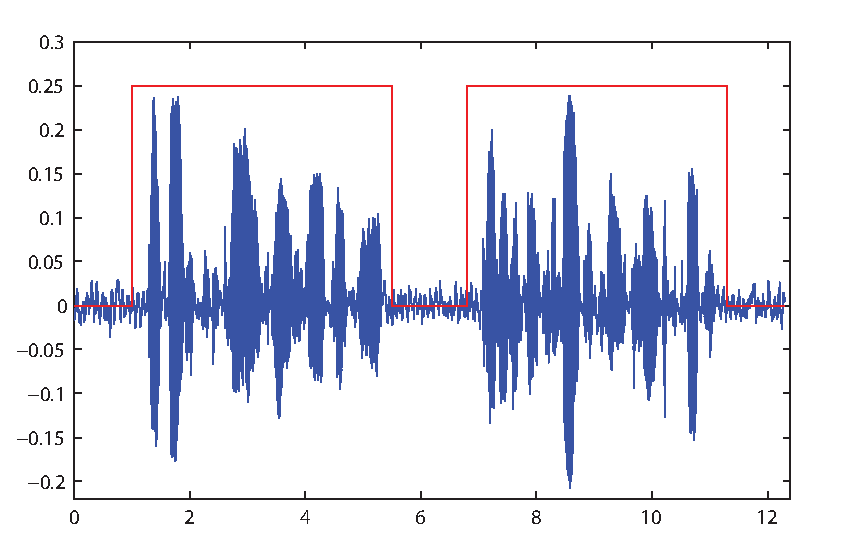
\includegraphics[width=0.9\columnwidth,keepaspectratio]{Figures/titlepage/titlepage.pdf}
%
%\vfill
%
%\setlength{\tabcolsep}{0pt}
%\begin{tabular}{p{40mm}p{\dimexpr\columnwidth-40mm}}
%Project Title: & \textbf{Robust Speech Detection in High Levels
%of Background Noise} \\[12pt]
%Student: & \href{mailto:marcin.baginski91@gmail.com}{\textbf{Marcin Baginski}} \\[12pt]
%CID: & \textbf{00656667} \\[12pt]
%Course: & \textbf{EIE4} \\[12pt]
%Project Supervisor: & \href{mailto:mike.brookes@imperial.ac.uk}{\textbf{Mr Mike Brookes}} \\[12pt]
%Second Marker: & \href{mailto:patrick.naylor@imperial.ac.uk}{\textbf{Dr Patrick Naylor}} \\
%\end{tabular}
%\end{titlepage}

%----------------------------------------------------------------------------------------
%	PAGE INTENTIONALLY LEFT BLANK
%----------------------------------------------------------------------------------------

%\newpage
%\thispagestyle{empty}
%\vspace*{120pt}
%
%\begin{center}
%\Large
% 
%\end{center}
%
%\clearpage

%----------------------------------------------------------------------------------------
%	ACTUAL TITLE PAGE
%----------------------------------------------------------------------------------------

\begin{titlepage}
\begin{center}

\includegraphics[scale=0.1]{Logo} % University/department logo - uncomment to place it 

\textsc{\LARGE \univname}\\[1cm] % University name
\textsc{\Large Final Year Project}\\[0.5cm] % Thesis type

\HRule \\[0.4cm] % Horizontal line
{\huge \bfseries \ttitle}\\[0.1cm] % Thesis title
\HRule \\[1.5cm] % Horizontal line
 
\begin{minipage}{0.4\textwidth}
\begin{flushleft} \large
\emph{Author:}\\
\href{mailto:marcin.baginski91@gmail.com}{\authornames} % Author name - remove the \href bracket to remove the link
\end{flushleft}
\end{minipage}
\begin{minipage}{0.4\textwidth}
\begin{flushright} \large
\emph{Supervisor:} \\
\href{mailto:mike.brookes@imperial.ac.uk}{\supname} % Supervisor name - remove the \href bracket to remove the link
%\emph{Second marker:} \\
%\href{mailto:patrick.naylor@imperial.ac.uk}{\secmark}
\end{flushright}
\end{minipage}\\[2cm]
 
\large This report is submitted in fulfilment of the requirements\\ for the degree of \textit{\degreename}\\ % University requirement text
in the\\
\deptname\\\univname\\[1.5cm] % Research group name and department name

{\large \today}\\[0.1cm] % Date

\vfill
\end{center}

\end{titlepage}

%----------------------------------------------------------------------------------------
%	PAGE INTENTIONALLY LEFT BLANK
%----------------------------------------------------------------------------------------

\newpage
\thispagestyle{empty}
\vspace*{120pt}

\begin{center}
\Large
 
\end{center}

\clearpage

%----------------------------------------------------------------------------------------
%	DECLARATION PAGE
%	Your institution may give you a different text to place here
%----------------------------------------------------------------------------------------

%\Declaration{
%
%\addtocontents{toc}{} % Add a gap in the Contents, for aesthetics
%
%I, \authornames, declare that this thesis titled, '\ttitle' and the work presented in it are my own. I confirm that:
%
%\begin{itemize} 
%\item[\tiny{$\blacksquare$}] Where any part of this thesis has previously been submitted for a degree or any other qualification at this University or any other institution, this has been clearly stated
%\item[\tiny{$\blacksquare$}] Where I have consulted the published work of others, this is always clearly attributed
%\item[\tiny{$\blacksquare$}] Where I have quoted from the work of others, the source is always given. With the exception of such quotations, this thesis is entirely my own work
%\item[\tiny{$\blacksquare$}] Where the thesis is based on work done by myself jointly with others, I have made clear exactly what was done by others and what I have contributed myself \medskip
%\end{itemize}
% 
%Signed:\\
%\rule[1em]{25em}{0.5pt} % This prints a line for the signature
% 
%Date:\\
%\rule[1em]{25em}{0.5pt} % This prints a line to write the date
%}
%
%\clearpage % Start a new page

%----------------------------------------------------------------------------------------
%	ABSTRACT PAGE
%----------------------------------------------------------------------------------------

\addtotoc{Abstract} % Add the "Abstract" page entry to the Contents

\abstract{\addtocontents{toc}{} % Add a gap in the Contents, for aesthetics

Voice Activity Detection (VAD) is a procedure of identifying speech segments within a recording. VAD is utilised in a variety of modern signal processing applications such as speech recognition, enhancement, transmission and coding. While VAD is a relatively simple task for clean recordings it becomes increasingly difficult as the power of the background noise rises. Over the recent years, researchers have proposed a number of approaches to VAD, however, the lack of standard methods for their evaluation makes it difficult to compare VAD algorithms objectively. This work contains a comprehensive literature survey of the existing VAD methods, their implementation as well as an objective evaluation through the use of identical test sets and unification of the algorithms' shared parts which could otherwise bias the results. Finally, an attempt to use one of the recently published pitch tracking algorithms as a Voice Activity Detector is described and its performance is examined. This approach has been shown to considerably outperform (on average) the best performing VAD method from the previous evaluation at the very high background noise levels i.e. when the SNR is in the range -5 to -15 dB.
}

\clearpage % Start a new page

%----------------------------------------------------------------------------------------
%	PAGE INTENTIONALLY LEFT BLANK
%----------------------------------------------------------------------------------------

\newpage
\thispagestyle{empty}
\vspace*{120pt}

\begin{center}
\Large
 
\end{center}

\clearpage

%----------------------------------------------------------------------------------------
%	ACKNOWLEDGEMENTS
%----------------------------------------------------------------------------------------

\setstretch{1.3} % Reset the line-spacing to 1.3 for body text (if it has changed)

\acknowledgements{\addtocontents{toc}{\vspace{1em}} % Add a gap in the Contents, for aesthetics

Firstly, I would like to thank my supervisor Mr Mike Brookes for coming up with an idea for this project, his great explanations of some of the concepts as well as his guidance, effort and inspiration during the project work.

I would also like to thank Dr Pier Luigi Dragotti for his excellent delivery of the `Signals and Linear Systems' lectures which sparked my interest in the field of signal processing.

Finally, I would like to thank my parents, family and my great friends for their continuous support during the last four years. I would have never been able to complete my studies in London without you which I have stated to you personally countless times. Dzieki!

}
\clearpage % Start a new page

%----------------------------------------------------------------------------------------
%	LIST OF CONTENTS/FIGURES/TABLES PAGES
%----------------------------------------------------------------------------------------

\pagestyle{fancy} % The page style headers have been "empty" all this time, now use the "fancy" headers as defined before to bring them back

\lhead{\emph{Contents}} % Set the left side page header to "Contents"
\tableofcontents % Write out the Table of Contents

\lhead{\emph{List of Figures}} % Set the left side page header to "List of Figures"
\listoffigures % Write out the List of Figures

\lhead{\emph{List of Tables}} % Set the left side page header to "List of Tables"
\listoftables % Write out the List of Tables

%----------------------------------------------------------------------------------------
%	THESIS CONTENT - CHAPTERS
%----------------------------------------------------------------------------------------

\mainmatter % Begin numeric (1,2,3...) page numbering

\pagestyle{fancy} % Return the page headers back to the "fancy" style

% Include the chapters of the thesis as separate files from the Chapters folder
% Uncomment the lines as you write the chapters

% Chapter Template

\chapter{Introduction} % Main chapter title

\label{Chapter1} % Change X to a consecutive number; for referencing this chapter elsewhere, use \ref{ChapterX}

\lhead{Chapter 1. \emph{Introduction}} % Change X to a consecutive number; this is for the header on each page - perhaps a shortened title

%----------------------------------------------------------------------------------------
%	SECTION 1
%----------------------------------------------------------------------------------------

\section{Voice Activity Detection}

Voice Activity Detection (VAD) is a problem of separating parts of an audio recording which contain the presence of human voice from those which are only comprised of silence or the background noise. VAD is a trivial task in recordings which have high signal-to-noise (SNR) ratios, in which voice can be distinguished from noise simply by computing the short-time energy of all frames and setting an appropriate threshold for their classification. However, in real applications, the signal is almost always contaminated by some level of background noise which makes the VAD's performance to drop. VAD decision is especially difficult for the unvoiced phonemes \cite{Kondoz} whose spectrum contains no periodicity and is often similar to the one of white noise \cite{Michaelis}. \medskip

There has been an active research in the VAD area from as early as 1975, when Rabiner and Sambur \cite{RabinerSambur} proposed a VAD algorithm (then referred to as "algorithm for determining the endpoints of isolated utterances") based on the aforementioned short-time energy and the zero-crossing rate. This approach worked reasonably well for signals with SNR ratio on the order of 30 dB, however since then there has been a need for much better performance, including applications where algorithm robustness has to be achieved even at negative SNRs.

%----------------------------------------------------------------------------------------
%	SECTION 2
%----------------------------------------------------------------------------------------

\section{Applications}

VAD is often a first step in many signal processing applications including speech recognition \cite{RamirezGorriz}, speech coding \cite{Sohn}, speech enhancement \cite{Park} or noise estimation \cite{RamirezGorriz}. \medskip

In Automatic Speech Recognition (ASR), it is important to first extract the voice-active parts of a signal and then pass them to the actual recognition module. This procedure increases both the accuracy of the ASR system as well as its speed, since the recognition task is not performed on the parts of the signal which do not contain speech. An example structure of a ASR system which uses VAD module is presented in Figure \ref{fig:ASRVAD} \cite{RamirezGorriz}. For this application, it is most important for the VAD module to be able to identify all speech segments, even if some of the returned frames are false positives. Typically, there is a trade-off in VAD performance which can be characterised as maximising the precision of the VAD decisions while keeping the recall at a high rate.\medskip

\begin{figure}[htbp]
	\centering
		\includegraphics[width=1\columnwidth]{Figures/ASRVAD.png}
		\rule{34em}{0.5pt}
	\caption[Block diagram of an ASR system which uses VAD as the first processing step]{Block diagram of an ASR system which uses VAD as the first processing step \cite{RamirezGorriz}}
	\label{fig:ASRVAD}
\end{figure}

Variable-rate speech coding techniques and discontinuous transmission (DTX) \cite{GSMControl} systems also benefit from robust Voice Activity Detection. For DTX, 
% Chapter Template

\chapter{Literature Survey of the VAD algorithms} % Main chapter title

\label{Chapter2} % Change X to a consecutive number; for referencing this chapter elsewhere, use \ref{ChapterX}

\lhead{Chapter 2. \emph{Literature Survey of the VAD algorithms}} % Change X to a consecutive number; this is for the header on each page - perhaps a shortened title

%----------------------------------------------------------------------------------------
%	SECTION 1 - Standard VAD algorithms
%----------------------------------------------------------------------------------------

\section{Standard VAD algorithms}

Being an important tool in many speech processing applications, a number of VAD algorithms have been subject to standardisation by various organisations such as the International Telecommunication Union (ITU-T), European Telecommunications Standards Institute (ETSI), Telecommunications Industry Association (TIA) or Electronic Industries Alliance (EIA). It is important to note that most of the standardised VAD approaches have been developed for use in the telecommunications industry, with particular emphasis on the application for discontinuous transmission (DTX), which may make them less appropriate for other speech processing tasks such as speech recognition.

In the rest of this chapter, three standard VAD algorithms are going to be described:
\begin{itemize}
\item ITU-T G.729 Annex B \citep{G729} which is an extension to the G.729 speech coder with an aim to achieve an improved bit rate during the noise-only periods
\item ETSI AMR1 and AMR2 \cite{AMR} for application to the Global System for Mobile Communications (GSM)
\item TIA/EIA IS-733 \cite{IS733} for application to the Wideband Spread Spectrum Communication Systems
\end{itemize}

\subsection{ITU-T G.729 Annex B}

The well-known ITU-T G.729 Annex B VAD has been developed as an extension to the G.729 speech coding algorithm \citep{G729Original} transmitting each frame at a fixed bit rate of 8 kb/s. Application of the Voice Activity Detector allows to identify the noise-only frames in a continuous stream of data and adopt a compressed transmission at only 15 b/frame which contains information about the background noise for reproduction by the Comfort Noise Generator (CNG) at the receiving end. This approach for speech/noise coding allows to reduce the average bit-rate of the entire coder from 8 kb/s to only 4 kb/s while keeping the transmission quality unchanged.

The block diagram of the VAD algorithm is presented in Figure \ref{fig:G729AnnexB}. It starts with computation of four main \emph{instantaneous parameters} for the current frame which describe the energy and spectral content of the signal:
\begin{itemize}
\item Set of Line Spectral Frequencies (LSF)
\item Full-band energy ($E_f$)
\item Low-band (0 to 1 kHz) energy ($E_l$)
\item Zero-crossing rate (ZCR)
\end{itemize}

\begin{figure}[htbp]
	\centering
		\includegraphics[width=0.9\columnwidth]{Figures/G729AnnexB.png}
		\rule{37em}{0.5pt}
	\caption[Block diagram of the ITU-T G.729 Annex B Voice Activity Detector]{Block diagram of the ITU-T G.729 Annex B Voice Activity Detector \cite{Kondoz}}
	\label{fig:G729AnnexB}
\end{figure}

The \emph{instantaneous parameters} are then differenced with their most recent average noise-only counterparts in order to derive an additional set of so called \emph{difference parameters} which are used for speech/non-speech classification. The set of all possible \emph{difference parameters} describes a four dimensional Euclidean space in which a specific region contains the speech frames while another region describes the noise-only frames. The current vector of parameters is compared against the pre-computed regions in order to classify the current frame. The two regions are initially identified by visual inspection of the points' distribution over a large set of clean and noisy recordings. An energy threshold of $E_f < 15 dB$ is applied before the multi-boundary classification in order to minimise short glitches on low-energy frames.

ITU-T G.729 Annex B uses an additional four-step heuristic-based smoothing scheme after the initial multi-boundary classification:
\begin{enumerate}
\item An active voice decision is extended to the current frame if its energy is above a certain threshold
\item An active voice decision is extended to the current frame if the previous two frames were speech and the absolute energy difference between the current and previous frames' is under a certain threshold
\item An inactive voice decision is extended to the current frame if the previous 10 frames were noise-only and the absolute energy difference between current and previous frames' is under a certain threshold
\item The active voice frame is labelled as inactive if the current frame energy is below a noise floor by a certain threshold
\end{enumerate}

The VAD algorithm also performs updates of the noise parameters ($\overline{LSF}$, $\overline{E_f}$, $\overline{E_l}$ , $\overline{ZCR}$) by a secondary VAD decision which does not need to be extremely robust since it is used only for noise parameters estimation.

\subsection{ETSI AMR1 and AMR2}

ETSI proposed two VAD alternatives for use in the Adaptive Multi-Rate speech traffic channels. In both algorithms, the decision is primarily based on the energy of the signal to be classified across different frequency bands.

The block diagram of the AMR Option 1 VAD is presented in Figure \ref{fig:AMR1}. The input signal is first passed through a series of band-pass filters which split the time-domain signal into different frequency bands based on the Table \ref{AMR1filterbank}.

\begin{table}[htbp]
\center
\begin{tabular}{c|c|}
\cline{2-2}
 & Frequencies \\ \hline
\multicolumn{1}{ |c| }{Bank 1} & 0 - 250 Hz \\ \hline
\multicolumn{1}{ |c| }{Bank 2} & 250 - 500 Hz \\ \hline
\multicolumn{1}{ |c| }{Bank 3} & 500 - 750 Hz \\ \hline
\multicolumn{1}{ |c| }{Bank 4} & 750 - 1000 Hz \\ \hline
\multicolumn{1}{ |c| }{Bank 5} & 1000 - 1500 Hz \\ \hline
\multicolumn{1}{ |c| }{Bank 6} & 1500 - 2000 Hz \\ \hline
\multicolumn{1}{ |c| }{Bank 7} & 2000 - 2500 Hz \\ \hline
\multicolumn{1}{ |c| }{Bank 8} & 2500 - 3000 Hz \\ \hline
\multicolumn{1}{ |c| }{Bank 9} & 3000 - 4000 Hz \\ \hline
\end{tabular}
\caption[Cut-off frequencies for the ETSI AMR1 band-pass filters]{Cut-off frequencies for the ETSI AMR1 band-pass filters \citep{AMR}}
\label{AMR1filterbank}
\end{table}

\begin{figure}[htbp]
	\centering
		\includegraphics[width=0.9\columnwidth]{Figures/AMR1.png}
		\rule{37em}{0.5pt}
	\caption[Block diagram of the ETSI AMR Option 1 Voice Activity Detector]{Block diagram of the ETSI AMR Option 1 Voice Activity Detector \cite{Kondoz}}
	\label{fig:AMR1}
\end{figure}



%\begin{figure}[htbp]
%	\centering
%		\includegraphics[width=0.9\columnwidth]{Figures/AMR2.png}
%		\rule{37em}{0.5pt}
%	\caption[Block diagram of the ETSI AMR Option 2 Voice Activity Detector]{Block diagram of the ETSI AMR Option 2 Voice Activity Detector \cite{Kondoz}}
%	\label{fig:AMR2}
%\end{figure}

\subsection{TIA/EIA IS-733}

%----------------------------------------------------------------------------------------
%	SECTION 2 - Other VAD algorithms
%----------------------------------------------------------------------------------------

\section{Other VAD algorithms}
% Chapter Template

\chapter{Evaluation of VAD algorithms} % Main chapter title

\label{Chapter3} % Change X to a consecutive number; for referencing this chapter elsewhere, use \ref{ChapterX}

\lhead{Chapter 3. \emph{Evaluation of VAD algorithms}} % Change X to a consecutive number; this is for the header on each page - perhaps a shortened title

%----------------------------------------------------------------------------------------
%	SECTION 1 - 
%----------------------------------------------------------------------------------------

\section{VAD evaluation methods}

Voice Activity Detection is a binary classification problem for which a number of standard evaluation methods are typically used...

\section{Preparation}

\subsection{Testing speech and noise}

\subsection{Noise power scaling}

\subsection{VAD implementation details}

\section{Evaluation results}

\section{Discussion}

\section{Conclusion}
% Chapter Template

\chapter{Evaluation of VAD algorithms} % Main chapter title

\label{Chapter4} % Change X to a consecutive number; for referencing this chapter elsewhere, use \ref{ChapterX}

\lhead{Chapter 4. \emph{Evaluation of VAD algorithms}} % Change X to a consecutive number; this is for the header on each page - perhaps a shortened title

%------------------------------------------------
%	SECTION 1
%------------------------------------------------

\section{Main Section 1}

%------------------------------------------------
%	SECTION 1
%------------------------------------------------

\section{Main Section 2}

\begin{figure}[htbp]
	\centering
		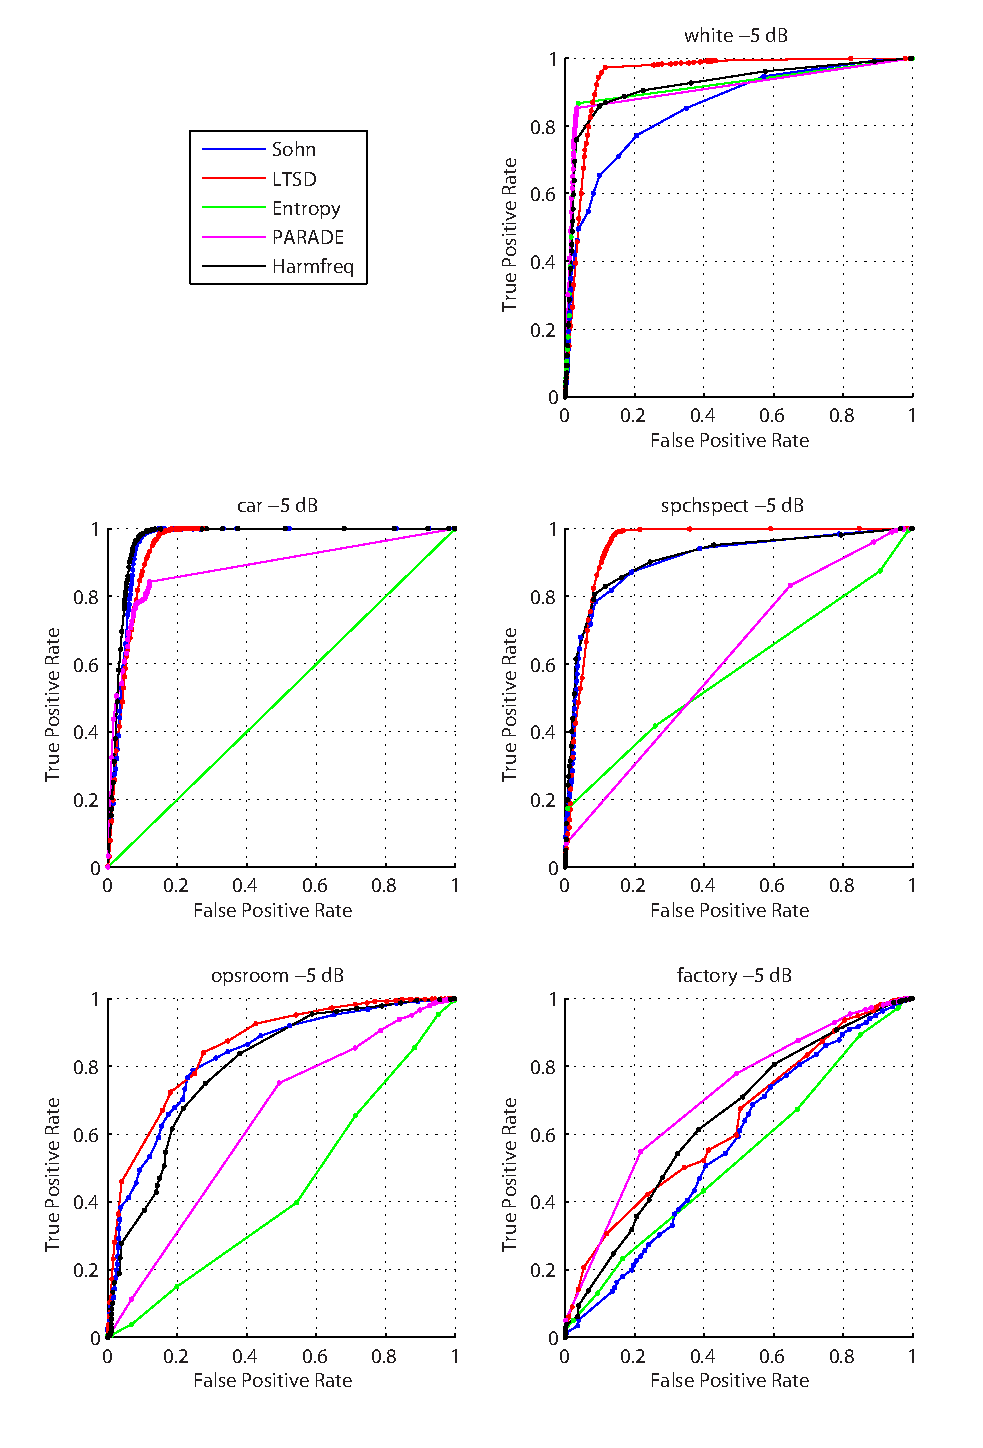
\includegraphics[width=1.0\columnwidth]{Figures/Chapter3/-5dBh.pdf}
		\rule{37em}{0.5pt}
	\caption[ROC curves of the evaluated algorithms \emph{with} hang-over under -5 dB SNR]{ROC curves of the evaluated VAD algorithms \emph{with} hang-over under -5 dB SNR}
	\label{fig:-5dBh}
\end{figure}

\begin{table}[htbp]
\center
\begin{tabular}{c|c|c|c|c|c!{\vrule width 1.5pt}c|}
\cline{2-7}
 & white & car & spchspect & opsroom & factory & average \\ \hline
\multicolumn{1}{ |c| }{Sohn} & 0.8561 & 0.9595 & 0.9063 & 0.8276 & 0.5671 & 0.8233\\ \hline
\multicolumn{1}{ |c| }{LTSD} & \textcolor{LimeGreen}{0.9497} & 0.9496 & \textcolor{LimeGreen}{0.9502} & \textcolor{LimeGreen}{0.8586} & 0.6345 & \textcolor{LimeGreen}{\textbf{0.8685}}\\ \hline
\multicolumn{1}{ |c| }{Entropy} & 0.9160 & \textcolor{red}{0.4999} & \textcolor{red}{0.5807} & \textcolor{red}{0.4350} & \textcolor{red}{0.5315} & \textcolor{red}{\textbf{0.5926}}\\ \hline
\multicolumn{1}{ |c| }{PARADE} & \textcolor{red}{0.9117} & 0.8853 & 0.6159 & 0.6339 & \textcolor{LimeGreen}{0.7071} & 0.7508\\ \hline
\multicolumn{1}{ |c| }{Harmfreq} & 0.9209 & \textcolor{LimeGreen}{0.9676} & 0.9126 & 0.7992 & 0.6425 & 0.8486\\ \hline
\end{tabular}
\caption[AUC values of the evaluated algorithms \emph{with} hang-over under -5 dB SNR]{AUC values of the evaluated VAD algorithms \emph{with} hang-over under -5 dB SNR}
\label{tab:AUC-5dBh}
\end{table}

\begin{figure}[htbp]
	\centering
		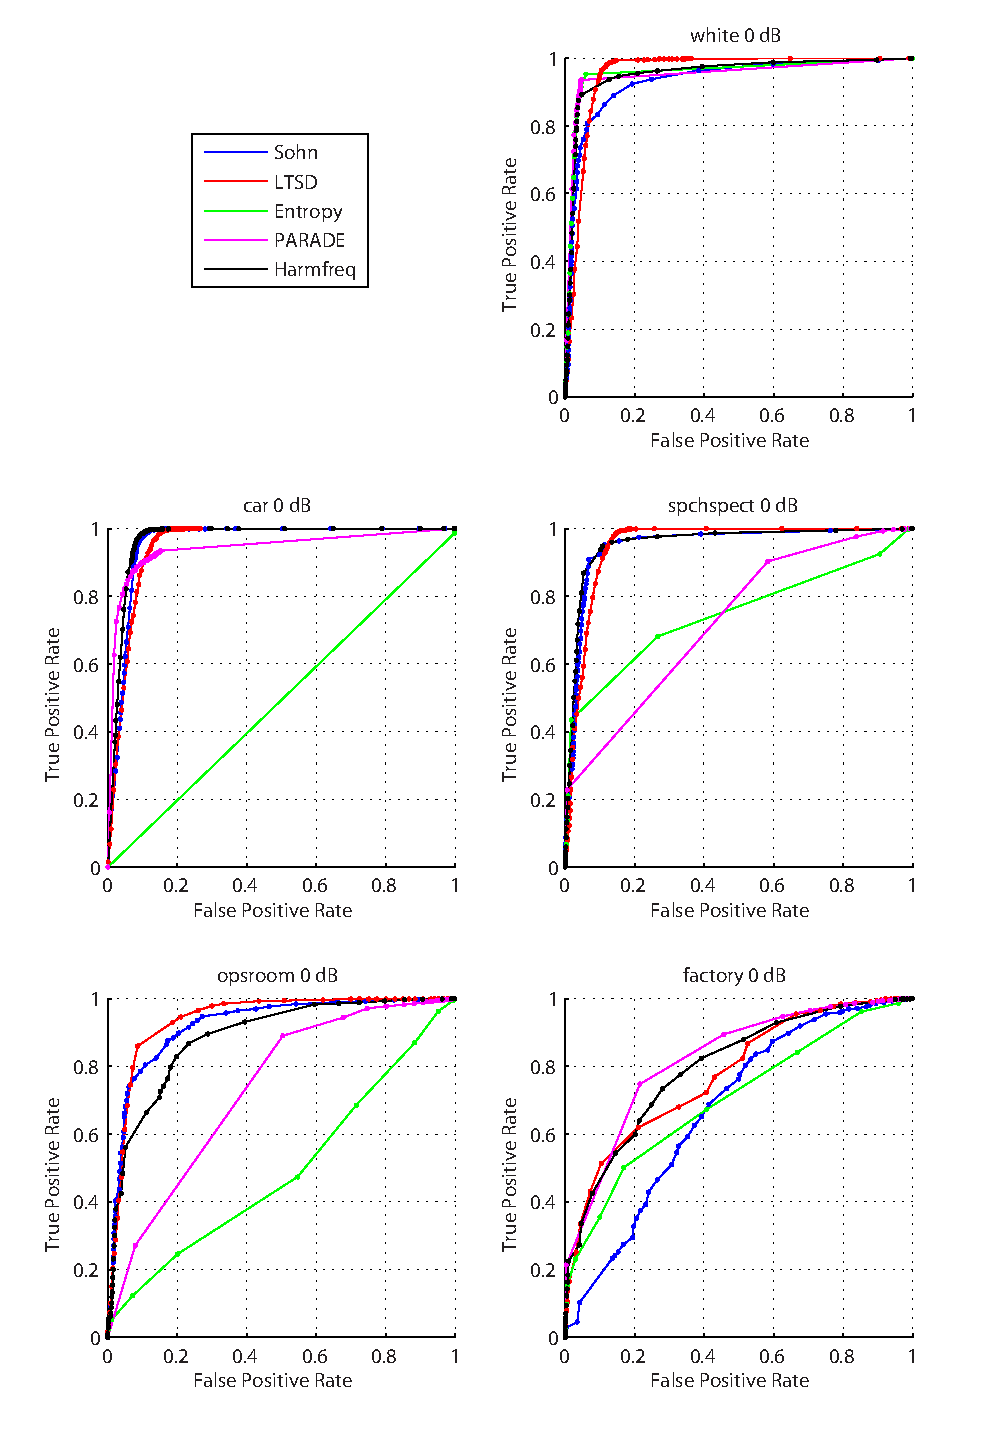
\includegraphics[width=1.0\columnwidth]{Figures/Chapter3/0dBh.pdf}
		\rule{37em}{0.5pt}
	\caption[ROC curves of the evaluated algorithms \emph{with} hang-over under 0 dB SNR]{ROC curves of the evaluated VAD algorithms \emph{with} hang-over under 0 dB SNR}
	\label{fig:0dBh}
\end{figure}

\begin{table}[htbp]
\center
\begin{tabular}{c|c|c|c|c|c!{\vrule width 1.5pt}c|}
\cline{2-7}
 & white & car & spchspect & opsroom & factory & average \\ \hline
\multicolumn{1}{ |c| }{Sohn} & \textcolor{red}{0.9334} & 0.9573 & 0.9506 & 0.9226 & \textcolor{red}{0.6740} & 0.8876\\ \hline
\multicolumn{1}{ |c| }{LTSD} & 0.9555 & 0.9498 & \textcolor{LimeGreen}{0.9508} & \textcolor{LimeGreen}{0.9390} & 0.7770 & \textcolor{LimeGreen}{\textbf{0.9144}}\\ \hline
\multicolumn{1}{ |c| }{Entropy} & \textcolor{LimeGreen}{0.9564} & \textcolor{red}{0.4942} & 0.7466 & \textcolor{red}{0.4926} & 0.7030 & \textcolor{red}{\textbf{0.6785}}\\ \hline
\multicolumn{1}{ |c| }{PARADE} & 0.9513 & 0.9415 & \textcolor{red}{0.7267} & 0.7329 & \textcolor{LimeGreen}{0.8225} & 0.8350\\ \hline
\multicolumn{1}{ |c| }{Harmfreq} & 0.9541 & \textcolor{LimeGreen}{0.9673} & 0.9557 & 0.8862 & 0.7976 & 0.9122\\ \hline
\end{tabular}
\caption[AUC values of the evaluated algorithms \emph{with} hang-over under 0 dB SNR]{AUC values of the evaluated VAD algorithms \emph{with} hang-over under 0 dB SNR}
\label{tab:AUC0dBh}
\end{table}

\begin{figure}[htbp]
	\centering
		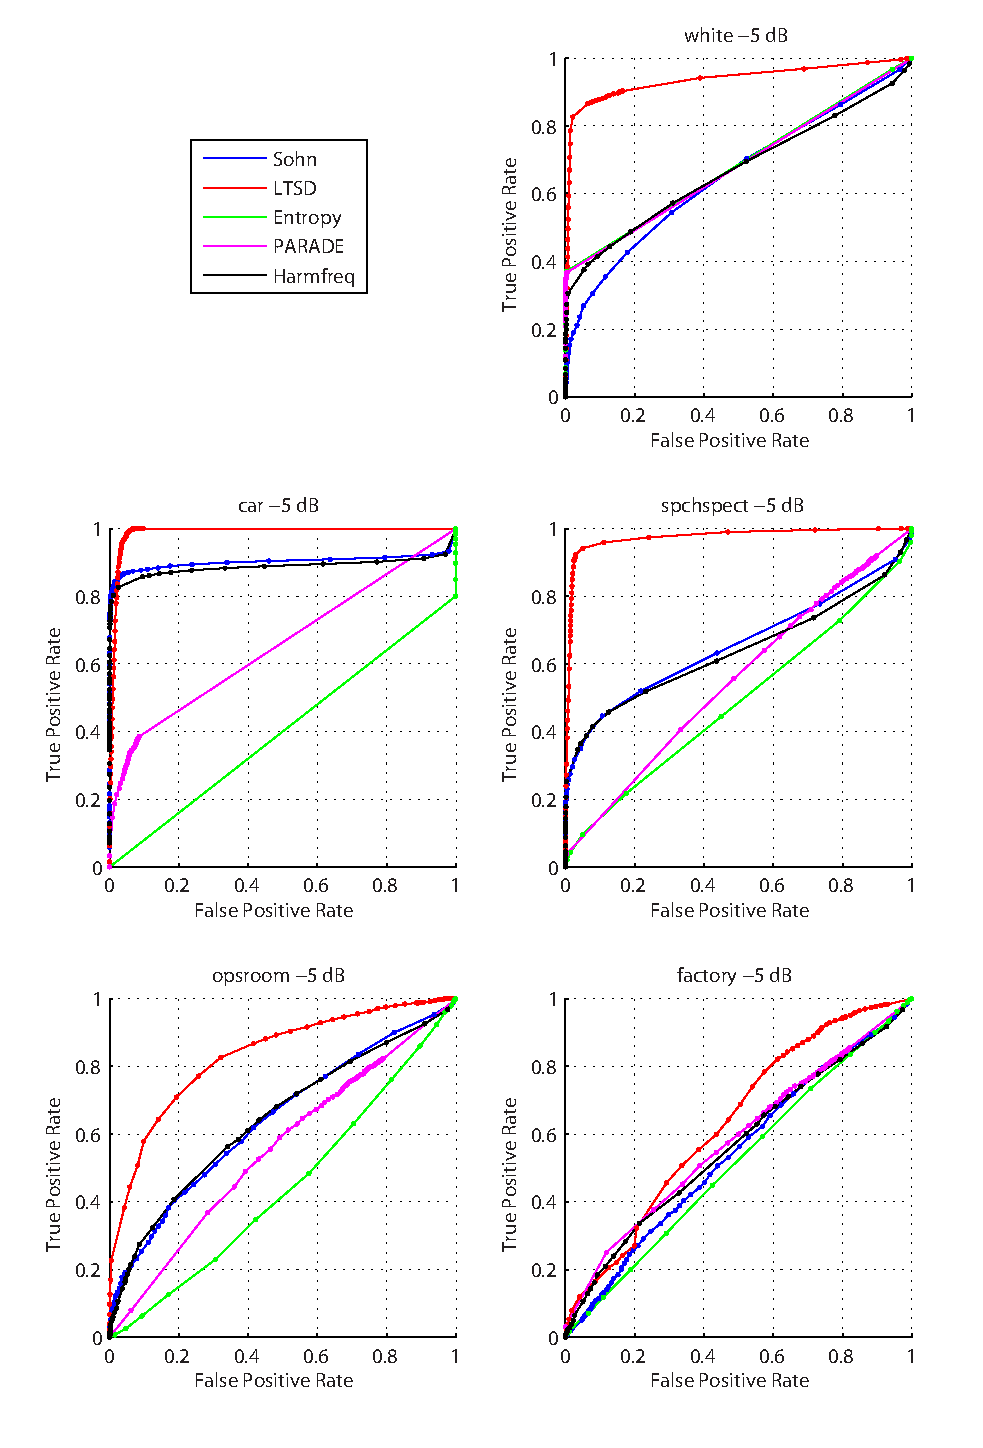
\includegraphics[width=1.0\columnwidth]{Figures/Chapter3/-5dBnoh.pdf}
		\rule{37em}{0.5pt}
	\caption[ROC curves of the evaluated algorithms \emph{without} hang-over under -5 dB SNR]{ROC curves of the evaluated VAD algorithms \emph{without} hang-over under -5 dB SNR}
	\label{fig:-5dBnoh}
\end{figure}

\begin{figure}[htbp]
	\centering
		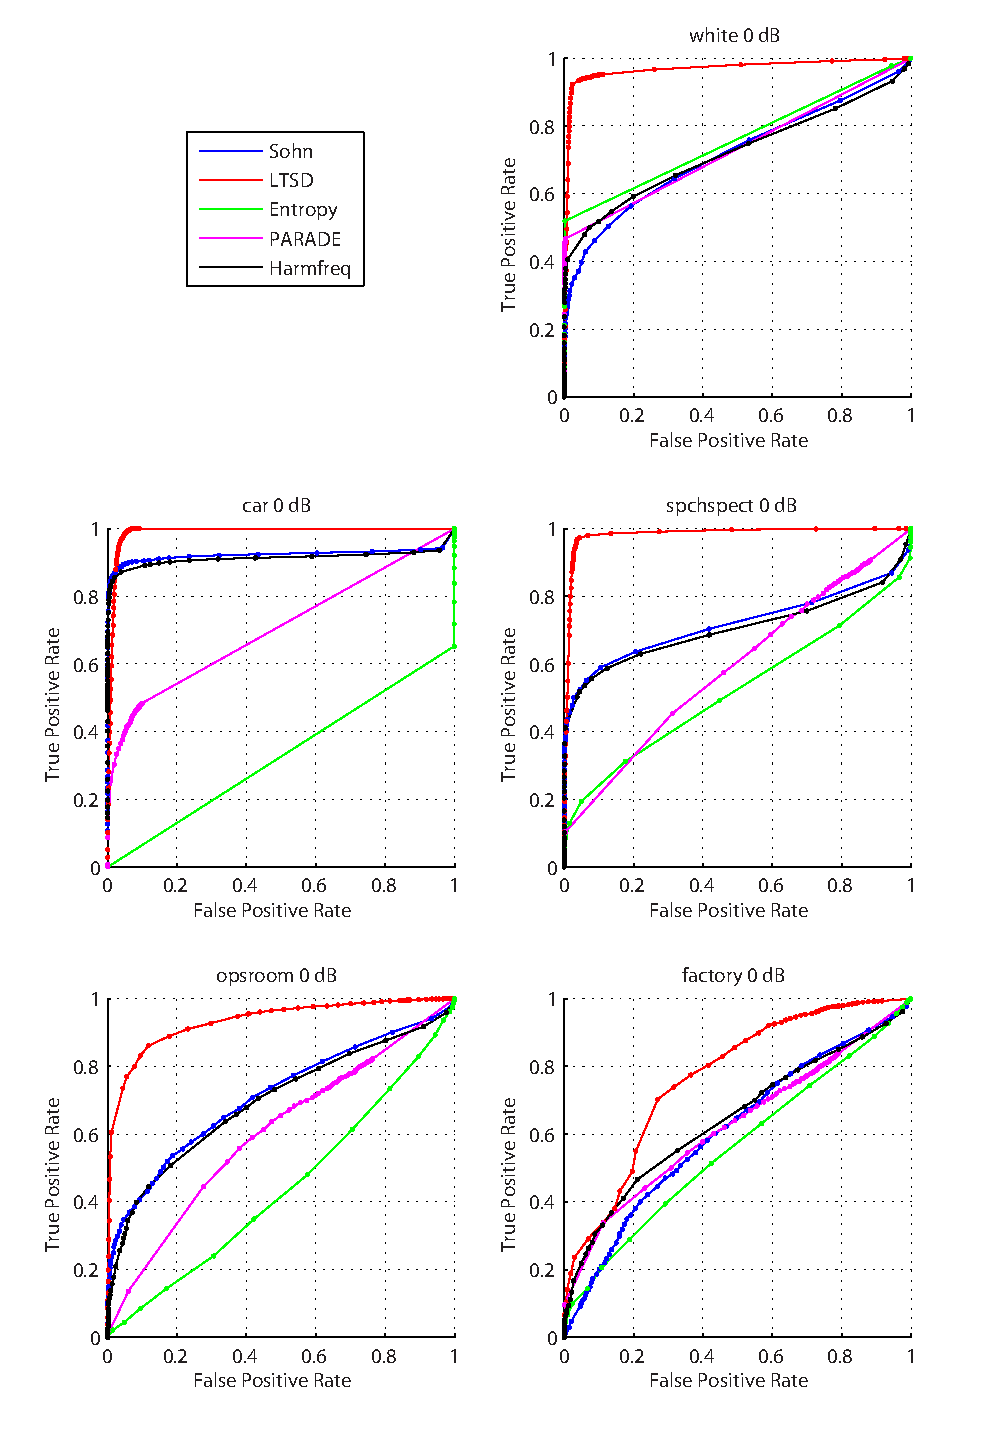
\includegraphics[width=1.0\columnwidth]{Figures/Chapter3/0dBnoh.pdf}
		\rule{37em}{0.5pt}
	\caption[ROC curves of the evaluated algorithms \emph{without} hang-over under 0 dB SNR]{ROC curves of the evaluated VAD algorithms \emph{without} hang-over under 0 dB SNR}
	\label{fig:0dBnoh}
\end{figure}
% Chapter Template

\chapter{An approach to VAD using PEFAC} % Main chapter title

\label{Chapter5} % Change X to a consecutive number; for referencing this chapter elsewhere, use \ref{ChapterX}

\lhead{Chapter 5. \emph{An approach to VAD using PEFAC}} % Change X to a consecutive number; this is for the header on each page - perhaps a shortened title

%----------------------------------------------------------------------------------------
%	SECTION 1 - PEFAC pitch tracker
%----------------------------------------------------------------------------------------

\section{PEFAC pitch tracker}

PEFAC pitch tracker \cite{PEFAC} is one of the recently published, robust pitch tracking algorithms which has been reported to achieve good results even at negative signal to noise ratios. Apart from calculating the pitch estimate as its primary output, it has also been designed to estimate the probability of a given frame \emph{being voiced} which is essentially a voiced speech activity detector. This value can be used to detect the voiced parts of a speech utterance by simple thresholding. Subsequent application of a hang-over scheme from Chapter \ref{Chapter3} should help in detecting the unvoiced segments. A combination of a thresholding stage and the hang-over scheme therefore creates a complete Voice Activity Detector.

The rest of this chapter is organised as follows. Firstly, an overview of PEFAC is presented. Then, the proposed approach to VAD is described in more detail, implemented and evaluated against LTSD, which was the best performing VAD from chapter \ref{Chapter4}. The experimental set-up for evaluation of PEFAC as VAD is the same as described in chapter \ref{Chapter3}.

%-----------------------------------
%	SUBSECTION 1 - PEFAC algorithm description
%-----------------------------------

\subsection{PEFAC algorithm description}

A detailed description of PEFAC is available in \cite{PEFAC}. The algorithm can however be summarised in the following steps:
\begin{enumerate}
\item Transform the input signal to the power spectrum domain using short-time Fourier transform
\item Interpolate the periodogram of each frame onto a log-spaced frequency grid
\item Calculate the normalized periodogram
\item Convolve the normalized periodogram with a comb filter in order to enhance speech harmonics and attenuate the noise
\item Select the three highest peaks in the feasible range as the initial pitch candidates
\item Estimate the probability of a frame being voiced
\item Use dynamic programming to identify the final pitch estimate
\end{enumerate}

The probability of a frame being voiced is based on two features:
\begin{enumerate}
\item The log-mean power of a frame $L_t = \log E_t$ such that $E_t = \frac{1}{Q} \sum_{n=1}^{Q} Y_t(q_i)$ where $Q$ is the number of frequency bins, $Y_t(q)$ is the normalized log-frequency periodogram. Using the log-mean power is justified since voiced speech typically contains most energy contained in a complete speech utterance and its mean power is therefore higher than that of unvoiced speech
\item The ratio of the sum of the highest three peaks in the spectrum convolved with the comb filter to $E_t$. Voiced speech contains most of its power in the harmonic bins therefore using this measure as a second feature is justified
\end{enumerate}

%----------------------------------------------------------------------------------------
%	SECTION 2
%----------------------------------------------------------------------------------------

\section{The proposed approach}

The proposed approach is relatively simple. PEFAC returns the probability of the current frame being voiced in a typical manner, i.e. as a number in the range 0 to 1. This can easily be thresholded and the voiced frames can be identified at this step. As stated numerously in the previous chapters, the voiced frames are typically surrounded by the unvoiced ones, hence application of the hang-over scheme from section \ref{sec:hang} will help to detect them. On average, this approach should perform well in detection of both the voiced as well as unvoiced phonemes which is the aim of a complete Voice Activity Detector.

%----------------------------------------------------------------------------------------
%	SECTION 3 - Evaluation results
%----------------------------------------------------------------------------------------

\section{Evaluation results}

The proposed approach has been implemented, evaluated and compared with the LTSD VAD. In all experiments, the hang-over scheme (section \ref{sec:hang}) has been applied to both algorithms. The evaluation of PEFAC without it does not make much sense, since by design it does not detect unvoiced phonemes and do they need to be identified by a secondary method. Other than that, the evaluation metrics are the same as in Chapter \ref{Chapter4}, namely the ROC curves and speech/non-speech hit rates with a fixed threshold.

The ROC curves for PEFAC and LTSD for all six noise types and two SNR levels (-5 dB and -10 dB) are presented in Figures \ref{fig:pefacm5} and \ref{fig:pefacm10}. For the white, car and opsroom noises, the performance of both algorithms seems to be comparable. PEFAC clearly underperforms LTSD in the babble and spchspect noises, which is expected to some extent, since being primarily a pitch tracker, the babble noise is probably the most difficult noise in which such algorithm might operate. Interestingly, PEFAC is far superior to LTSD in thr factory noise and its performance is much better in both SNR levels.

\begin{figure}[htbp]
	\centering
		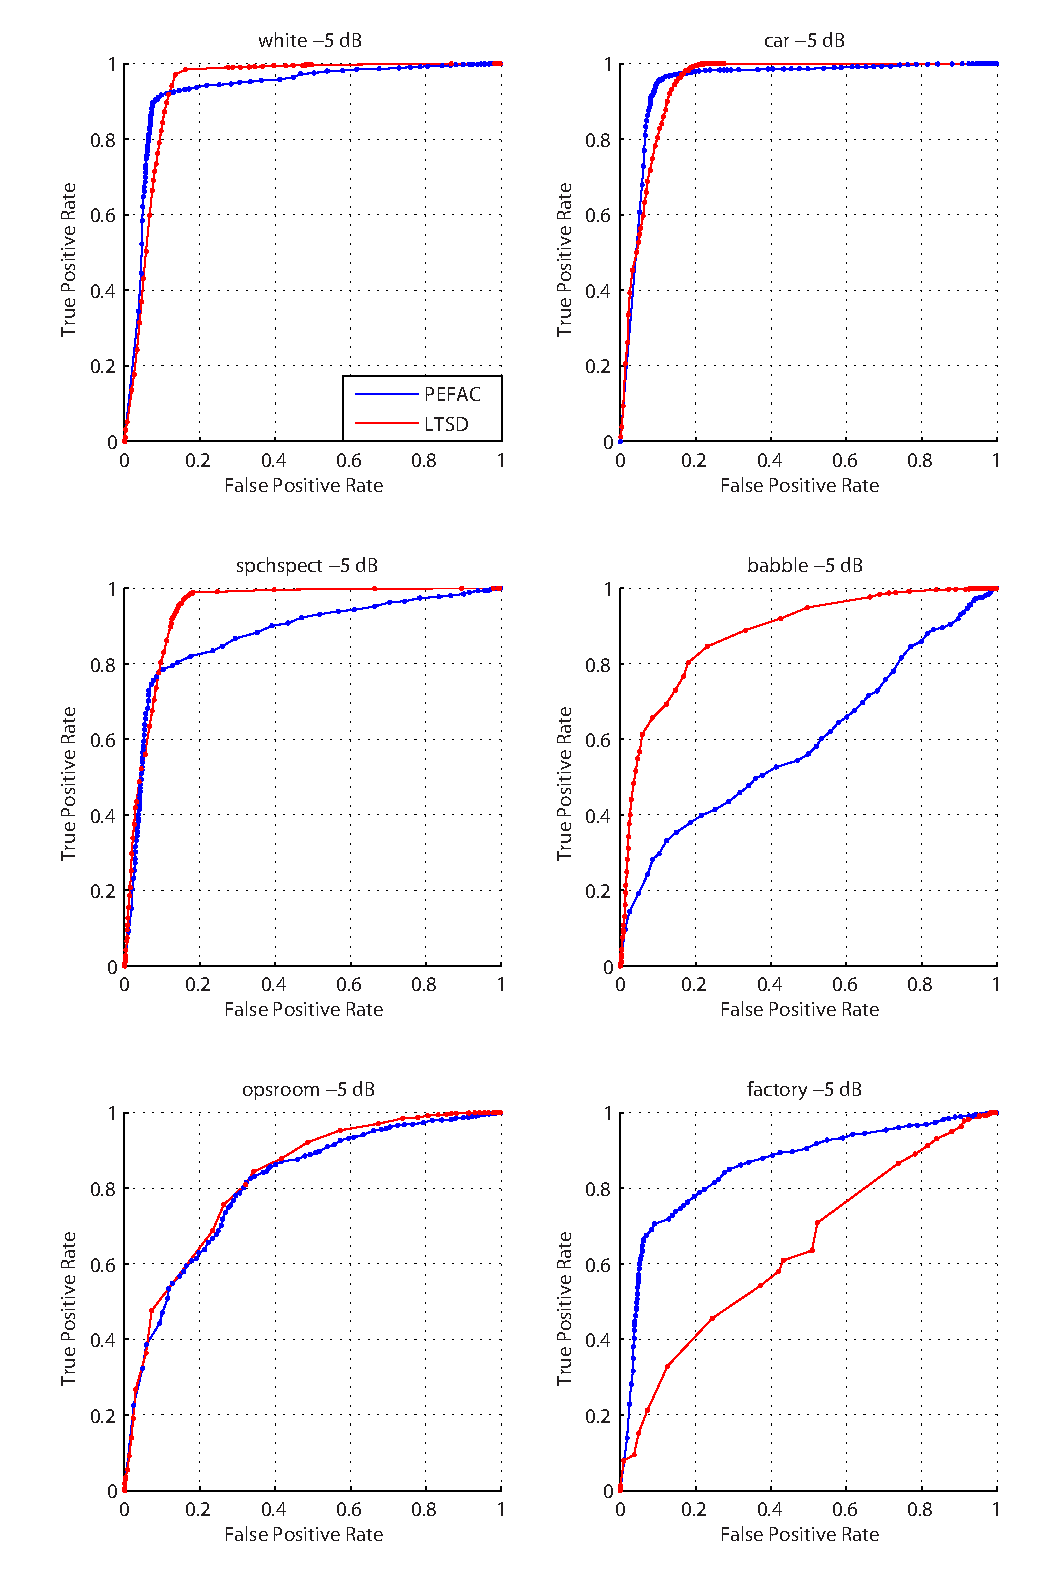
\includegraphics[width=1.0\columnwidth]{Figures/Chapter5/pefacm5.pdf}
		\rule{37em}{0.5pt}
	\caption[ROC curves of PEFAC and LTSD \emph{with} hang-over under -5 dB SNR]{ROC curves of PEFAC and LTSD \emph{with} hang-over under -5 dB SNR}
	\label{fig:pefacm5}
\end{figure}

\begin{figure}[htbp]
	\centering
		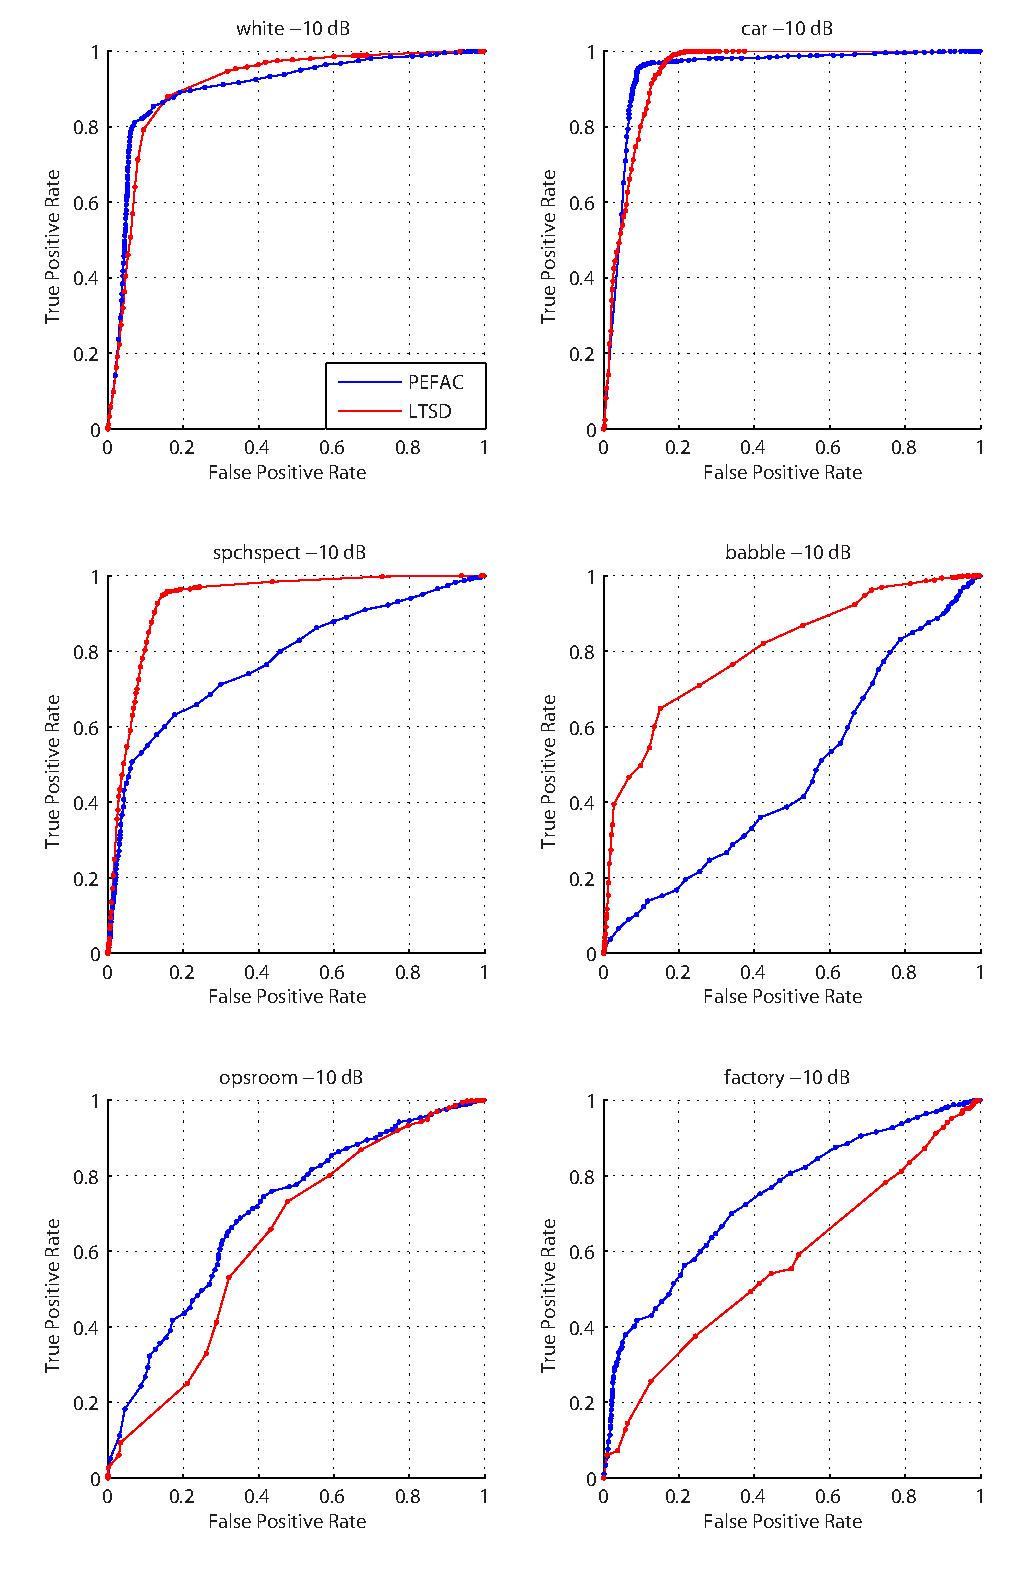
\includegraphics[width=1.0\columnwidth]{Figures/Chapter5/pefacm10.pdf}
		\rule{37em}{0.5pt}
	\caption[ROC curves of PEFAC and LTSD \emph{with} hang-over under -10 dB SNR]{ROC curves of PEFAC and LTSD \emph{with} hang-over under -10 dB SNR}
	\label{fig:pefacm10}
\end{figure}

The speech/non-speech hit rates with two fixed thresholds are presented in Figures \ref{fig:pefacSNR60} and \ref{fig:pefacSNR55}\footnote{The threshold in Figure \ref{fig:pefacSNR55} is lower than in \ref{fig:pefacSNR60} therefore a higher speech hit-rate but lower non-speech hit rate.}. Interestingly, for both threshold values PEFAC overperforms LTSD at low and very low SNRs i.e. in the range 0 to -15 dB. For the higher value of the fixed threshold (Figure \ref{fig:pefacSNR60}) PEFAC's performance is clearly better even in both speech and non-speech metrics while for the lower threshold, the non-speech hit rate at the low SNRs is very similar for both algorithms.

The slight disadvantage in the performance of PEFAC in the speech-hit rate at high SNRs comes from the parameters of the hang-over scheme. Specifically, sometimes the hang-over timer does is not long enough to capture all unvoiced beginnings or endings of speech utterances. This effect should be avoidable by making the frame length smaller and calibrating the hang-over parameters carefully.


\begin{figure}[htbp]
	\centering
		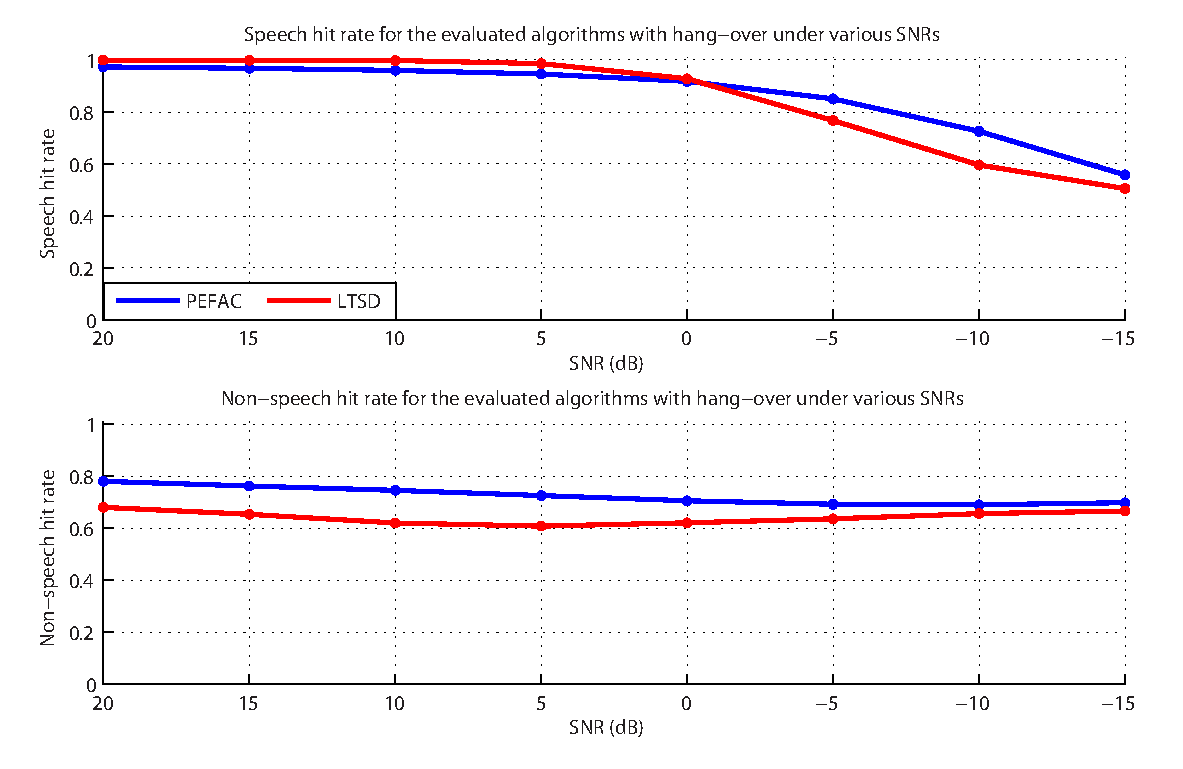
\includegraphics[width=0.81\columnwidth]{Figures/Chapter5/pefacSNR60bold.pdf}
		\rule{37em}{0.5pt}
	\caption[Speech/non-speech hit rates for PEFAC (higher threshold) and LTSD under different SNRs]{Speech/non-speech hit rates for PEFAC (higher threshold) and LTSD under different SNRs}
	\label{fig:pefacSNR60}
\end{figure}

\begin{figure}[htbp]
	\centering
		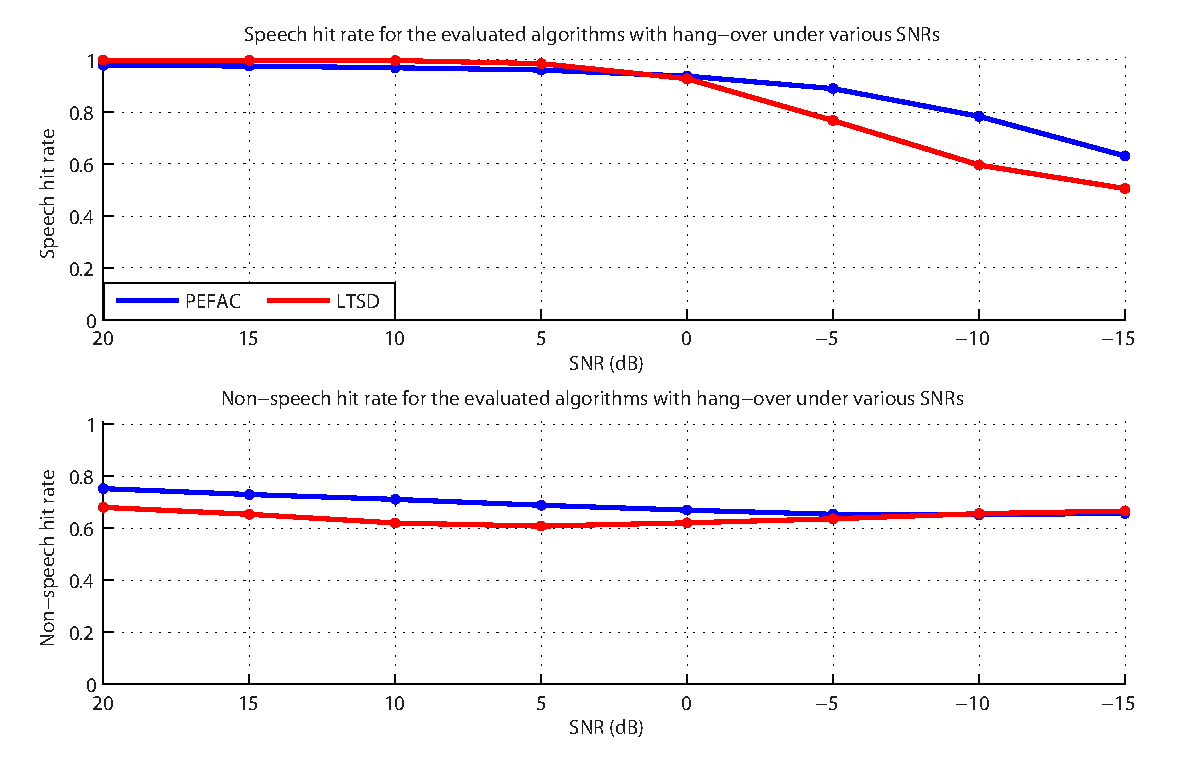
\includegraphics[width=0.81\columnwidth]{Figures/Chapter5/pefacSNR55bold.pdf}
		\rule{37em}{0.5pt}
	\caption[Speech/non-speech hit rates for PEFAC (lower threshold) and LTSD under different SNRs]{Speech/non-speech hit rates for PEFAC (lower threshold) and LTSD under different SNRs}
	\label{fig:pefacSNR55}
\end{figure}

\clearpage

%----------------------------------------------------------------------------------------
%	SECTION 4 - Summary
%----------------------------------------------------------------------------------------

\section{Summary}

The average performance of PEFAC is better than LTSD's at the very high SNR levels (-5 to -15 dB). This performance gain comes mostly from the much better operation in the factory noise and the fact that the best performance of PEFAC in all six noise types is achieved at similar threshold values (around 0.6) while for the LTSD algorithm the threshold values vary significantly between different noise types. Therefore, it can be concluded that PEFAC should be considered for applications which have to deal with varying conditions and high noise levels.
% Chapter Template

\chapter{Conclusions} % Main chapter title

\label{Chapter6} % Change X to a consecutive number; for referencing this chapter elsewhere, use \ref{ChapterX}

\lhead{Chapter 6. \emph{Conclusions}} % Change X to a consecutive number; this is for the header on each page - perhaps a shortened title

%---------------------------------------------------------------------
%	SECTION 1 - Project outcomes
%---------------------------------------------------------------------

\section{Project outcomes}

The project started with understanding the applications and a general structure of a VAD system (Chapter \ref{Chapter1}). During further literature survey (Chapter \ref{Chapter2}) it became clear that VAD is a very dispersed area of research and that a number of state-of-the-art algorithms exist. However, identification of the most noise-robust algorithm is difficult as the original performance results are not directly comparable. This motivated the creation of an artificial, yet identical for all algorithms, testing environment (Chapter \ref{Chapter3}) under which a few selected VAD methods could be objectively evaluated (Chapter \ref{Chapter4}). Finally, an approach to adapt one of the recently proposed pitch tracking algorithms to the area of VAD has been undertaken (Chapter \ref{Chapter5}).

The evaluation confirmed the initial hypothesis that the absolutely best VAD algorithm does not exist, as their performance often depends on the noise type and its power. Apart from that, the LTSD VAD achieved the best average results. For the very low SNRs and unknown or varying noise conditions the adaptation of PEFAC as VAD achieved promising evaluation results. Irrespective of the robustness of VAD features, all algorithms benefited significantly from a hang-over scheme applied to the initial VAD decisions.

%---------------------------------------------------------------------
%	SECTION 2 - Future work
%---------------------------------------------------------------------

\section{Future work}

Future work could be carried out in different areas. For starters, the speed of operation of the evaluated algorithms has not been taken into consideration. For some applications, such as real-time signal processing, this might be an important issue. Secondly, an evaluation on different, including some non-English, speech corpora and additional noise types could be performed.

A potentially interesting approach would be to examine using various VAD methods simultaneously in order to create a more noise-robust algorithm. The could be achieved either by forming a fusion of the decisions of various VAD methods or directing the operation of the composite algorithm by the identified noise type or the current SNR (i.e. using PEFAC when the estimated SNR is below 0 dB and LTSD otherwise). An obvious disadvantage of such noise-directed algorithm is the limited scope of operation. The decision fusion, on the other hand, could be created by assigning weights (which would need to be determined) to the outputs of various VAD methods.
%\input{Chapters/Chapter7}

%----------------------------------------------------------------------------------------
%	THESIS CONTENT - APPENDICES
%----------------------------------------------------------------------------------------

\addtocontents{toc}{\vspace{1em}} % Add a gap in the Contents, for aesthetics

\appendix % Cue to tell LaTeX that the following 'chapters' are Appendices

% Include the appendices of the thesis as separate files from the Appendices folder
% Uncomment the lines as you write the Appendices

% Appendix A

\chapter{Additional evaluation results} % Main appendix title

\label{AppendixA} % For referencing this appendix elsewhere, use \ref{AppendixA}

\lhead{Appendix A. \emph{Additional evaluation results}} % This is for the header on each page - perhaps a shortened title

This appendix contains the evaluation results for higher SNR levels than in the main body of the report, namely  5 dB and 10 dB SNR. In particular, the following figures are included below:

\begin{itemize}
\item Figure \ref{fig:5dBh} - ROC curves for 5 dB SNR, algorithms with hang-over
\item Figure \ref{fig:10dBh} - ROC curves for 10 dB SNR, algorithms with hang-over
\item Figure \ref{fig:5dBnoh} - ROC curves for 5 dB SNR, algorithms without hang-over
\item Figure \ref{fig:10dBnoh} - ROC curves for 10 dB SNR, algorithms without hang-over
\end{itemize}

\begin{figure}[htbp]
	\centering
		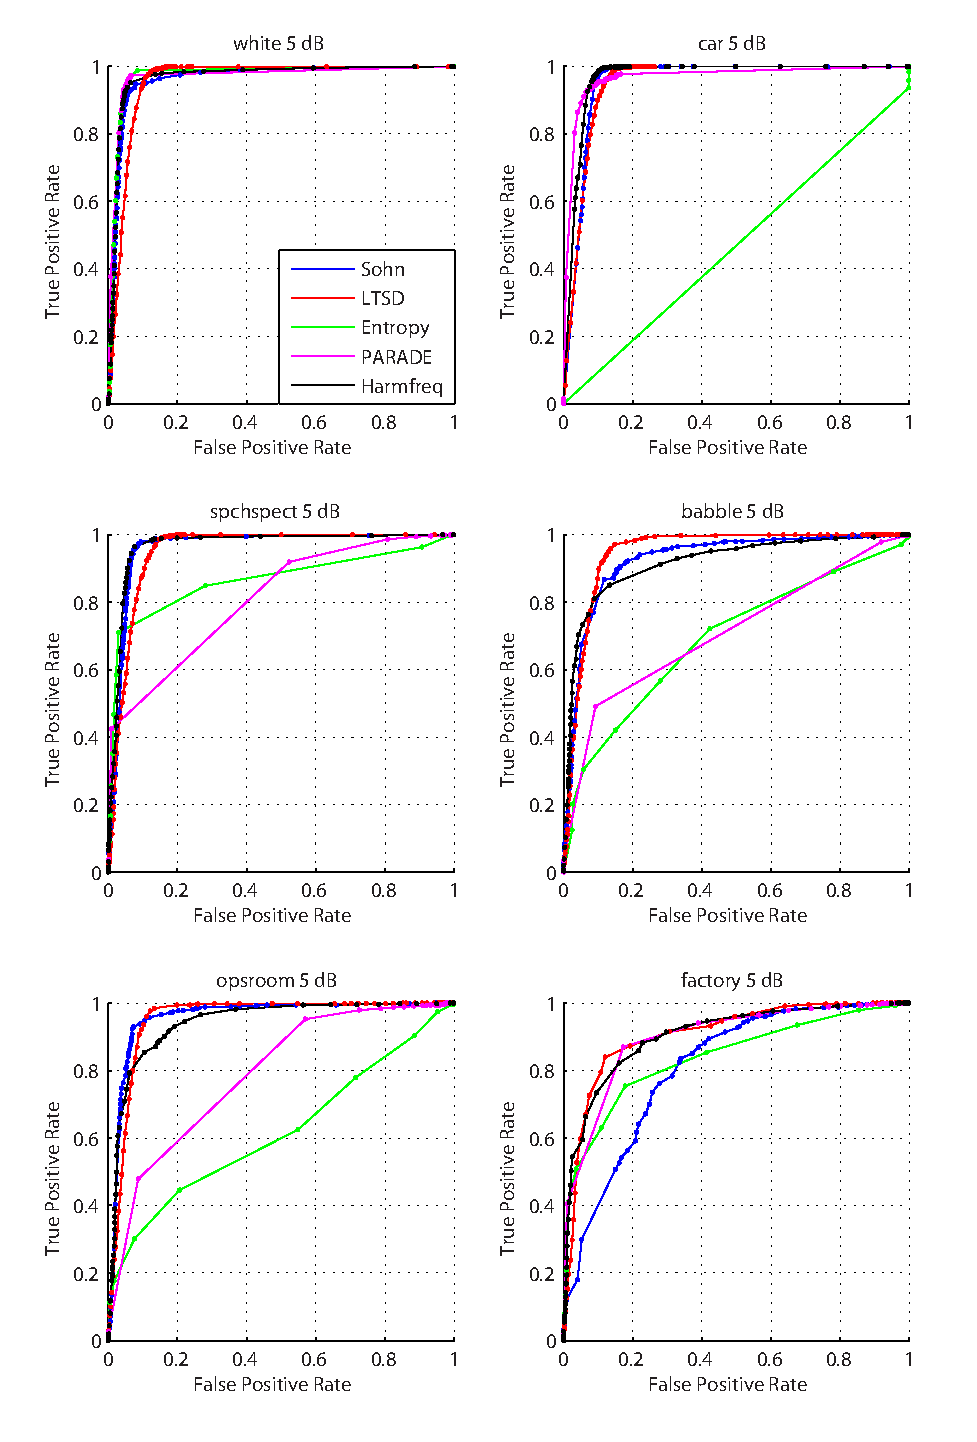
\includegraphics[width=1.0\columnwidth]{Figures/Chapter4/5dBh.pdf}
		\rule{37em}{0.5pt}
	\caption[ROC curves of the evaluated algorithms \emph{with} hang-over under 5 dB SNR]{ROC curves of the evaluated VAD algorithms \emph{with} hang-over under 5 dB SNR}
	\label{fig:5dBh}
\end{figure}

\begin{figure}[htbp]
	\centering
		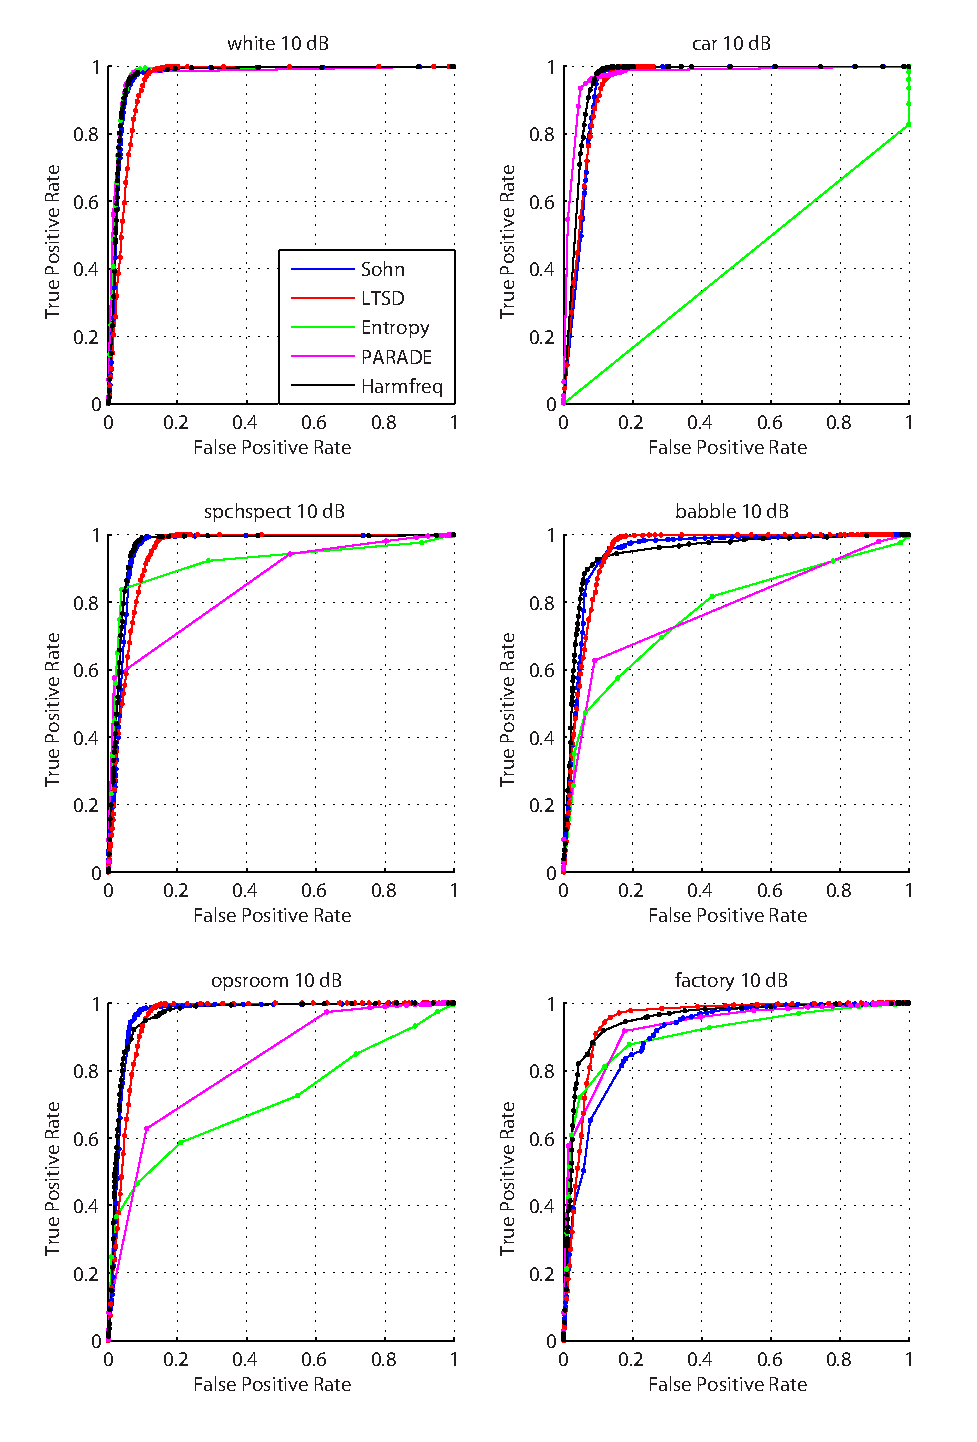
\includegraphics[width=1.0\columnwidth]{Figures/Chapter4/10dBh.pdf}
		\rule{37em}{0.5pt}
	\caption[ROC curves of the evaluated algorithms \emph{with} hang-over under 10 dB SNR]{ROC curves of the evaluated VAD algorithms \emph{with} hang-over under 10 dB SNR}
	\label{fig:10dBh}
\end{figure}

\begin{figure}[htbp]
	\centering
		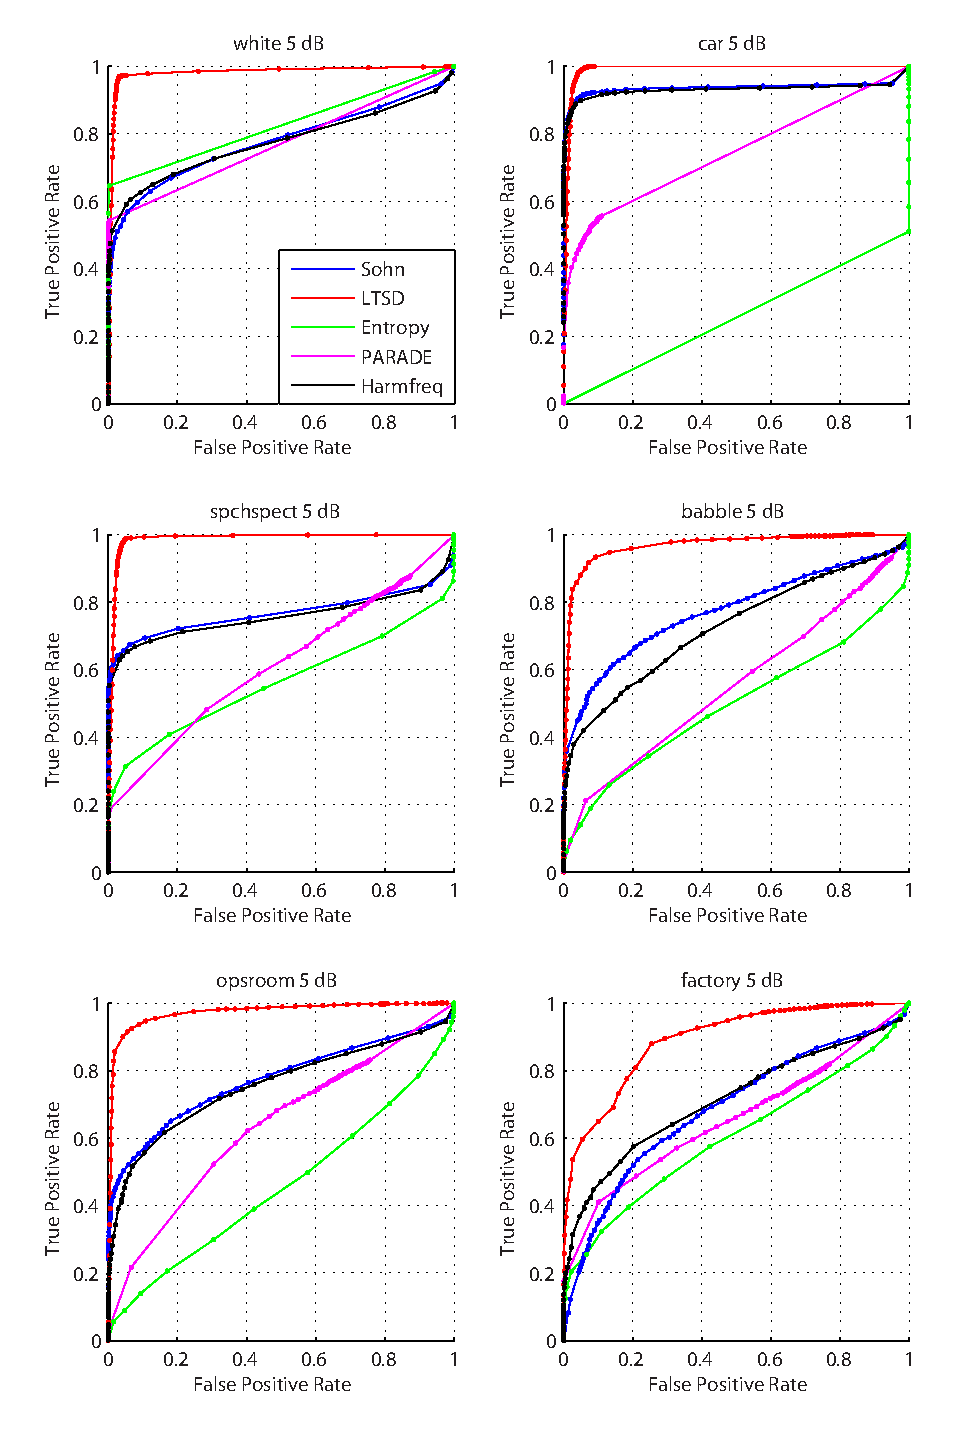
\includegraphics[width=1.0\columnwidth]{Figures/Chapter4/5dBnoh.pdf}
		\rule{37em}{0.5pt}
	\caption[ROC curves of the evaluated algorithms \emph{without} hang-over under 5 dB SNR]{ROC curves of the evaluated VAD algorithms \emph{without} hang-over under 5 dB SNR}
	\label{fig:5dBnoh}
\end{figure}

\begin{figure}[htbp]
	\centering
		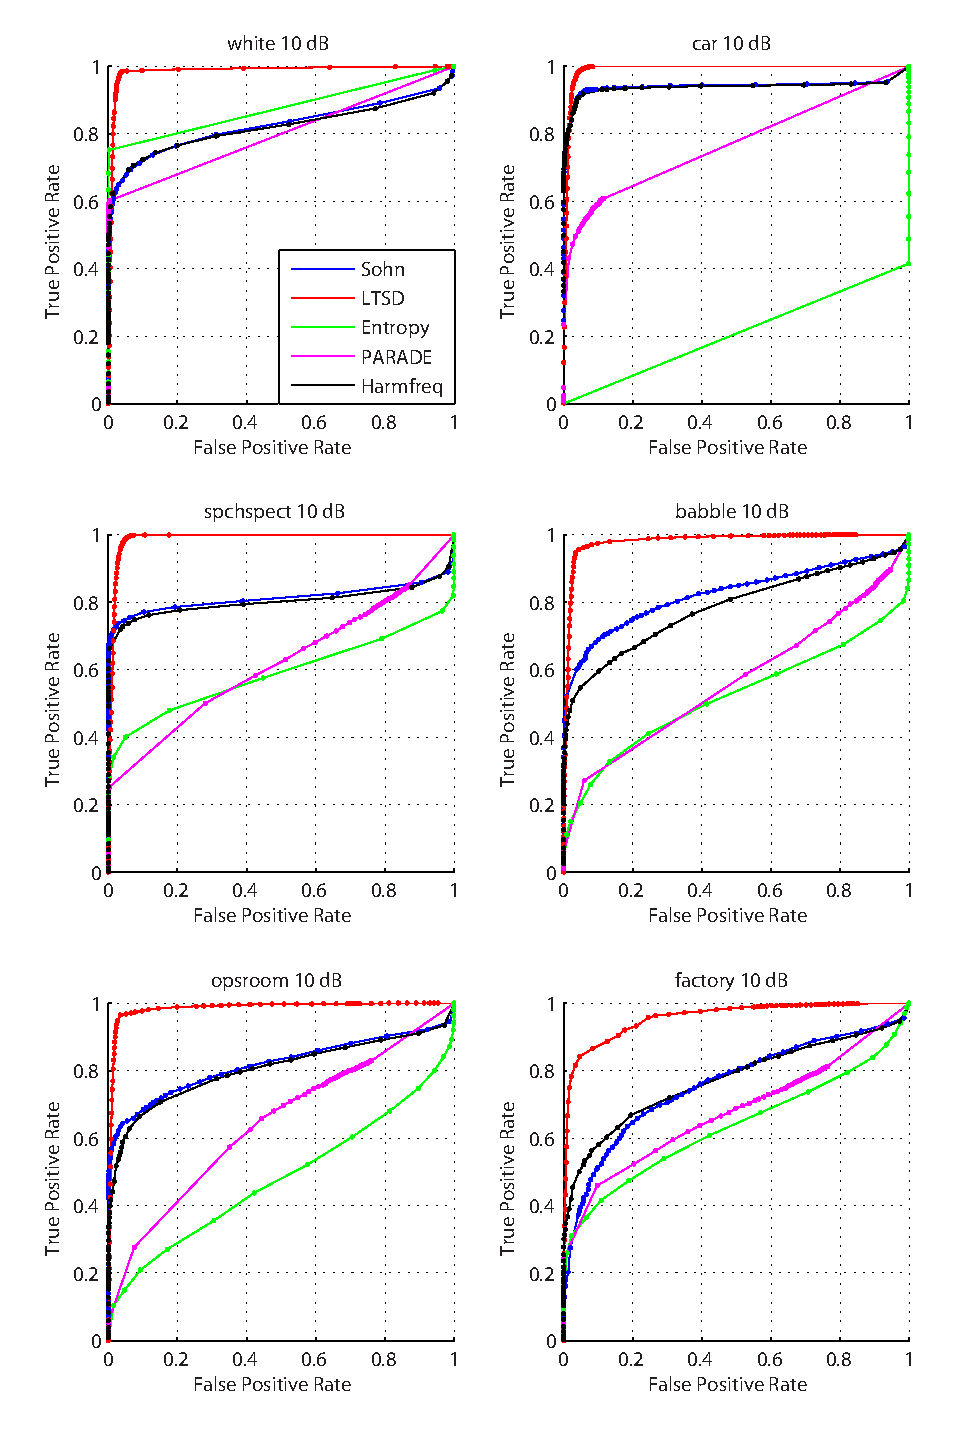
\includegraphics[width=1.0\columnwidth]{Figures/Chapter4/10dBnoh.pdf}
		\rule{37em}{0.5pt}
	\caption[ROC curves of the evaluated algorithms \emph{without} hang-over under 10 dB SNR]{ROC curves of the evaluated VAD algorithms \emph{without} hang-over under 10 dB SNR}
	\label{fig:10dBnoh}
\end{figure}
%\input{Appendices/AppendixB}
%\input{Appendices/AppendixC}

\addtocontents{toc}{\vspace{1em}} % Add a gap in the Contents, for aesthetics

\backmatter

%----------------------------------------------------------------------------------------
%	BIBLIOGRAPHY
%----------------------------------------------------------------------------------------

\label{Bibliography}

\lhead{\emph{Bibliography}} % Change the page header to say "Bibliography"

%\nocite{*} % Include also the uncited references

\bibliographystyle{unsrtnat} % Use the "unsrtnat" BibTeX style for formatting the Bibliography in alphabetical order

\bibliography{Bibliography} % The references (bibliography) information are stored in the file named "Bibliography.bib"

\end{document}  